\documentclass[border=10pt]{standalone}
%%%<
\usepackage{verbatim}
%%%>
\usepackage{pgfplots}
\pgfplotsset{width=7cm,compat=1.8}
\usepackage{pgfplotstable}
\begin{comment}
:Title: Differential equation direction plot
:Tags: 2D;PGFPlotstable;Mathematics
:Author: Jake
:Slug: differential-equation

Using PGFPlotstable, we can use a naive numerical integration
scheme to find the function directly within LaTeX.

This code was written by Jake on TeX.SE.
\end{comment}
\pgfplotstableset{
    create on use/x/.style={
        create col/expr={
            \pgfplotstablerow/201*2-1
        }
    },
    create on use/y/.style={
        create col/expr accum={
            \pgfmathaccuma+(2/201)*(abs(\pgfmathaccuma^2)+abs(\thisrow{x}^2)-1)
        }{0.6}
    },
        create on use/z/.style={
        create col/expr accum={
            \pgfmathaccuma+(2/201)*(abs(\pgfmathaccuma^2)+abs(\thisrow{y}^2)-1)
        }{0.6}
    }
    
}
\pgfplotstablenew{201}\loadedtable
\begin{document}
% Preamble: \pgfplotsset{width=7cm,compat=1.13}
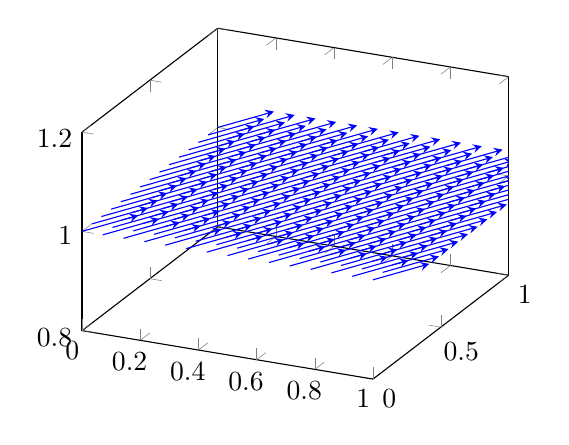
\begin{tikzpicture}
\begin{axis}[
domain=0:1,
xmax=1,
ymax=1
]
\addplot3[blue,/pgfplots/quiver,
quiver/u=1,
quiver/v=2,
quiver/w=0,
quiver/scale arrows=0.1,
-stealth,samples=15] {1};
\end{axis}
\end{tikzpicture}
\end{document}